% !TEX encoding = UTF-8 Unicode
%!TEX root = main.tex
% !TEX spellcheck = en-US
%%=========================================


%%%%%%%%%%%%%%%%%%%%%%%%%%%%%%%%%%%%%%%%%%%%%%%%%%%%%%%%%%%%%%%%%%%%%%%%%%%%%%%%
\chapter{Implementation}
\label{ch:implementation}


The library is written in C++, with standard C++14 dialect. The reader is expected to have a fair understanding of C++, and being familiar with standard C++11 dialect or newer is recommended. Detailed explanations of the C++ programming language is not presented here. Refer to any C++ reference (e.g. \citet{stroustrup2013c++}) for more details.


%%%%%%%%%%%%%%%%%%%%%%%%%%%%%%%%%%%%%%%%%%%%%%%%%%%%%%%%%%%%%%%%%%%%%%%%%%%%%%%%
\section{Data Structures}
\label{sec:data_structures}


A set of data structures is commonly used by the runtime system. Apart from the C++ Standard Template Library (STL), the most notable data structures are \textit{intrusive containers}, \textit{concurrent queues}, and \textit{mutual exclusion locks}.


%%%%%%%%%%%%%%%%%%%%%%%%%%%%%%%%%%%%%%%%
\subsection{Intrusive Containers and Pointers}


Intrusive containers, just as any other containers, stores some kind of data in some sort of way. The difference is how the container stores the necessary data used to organize the data. A non\hyp{}intrusive container is responsible for storing the necessary data, while for an intrusive container the elements are responsible for storing the necessary data. In other words, the element becomes ``aware'' of being a part of the intrusive container. Usually, intrusive containers are implemented with the elements having \textit{hooks} as data members. These hooks contains all the necessary data used by the intrusive container to store the elements. 

An intrusive pointer is the intrusive equivalent of a smart pointer with shared ownership, releasing a dynamically allocated object when all owners have released the pointer. The owner counter is stored in the object rather in the pointer.

Intrusive containers and pointers offers better performance compared to non\hyp{}intrusive containers, as they minimize memory allocations and better memory locality. Intrusive containers and pointers are however much less maintainable, and are much harder to modularize.

Boost Intrusive containers and Boost Intrusive pointers are used as the implementation of intrusive containers and pointers.


%%%%%%%%%%%%%%%%%%%%%%%%%%%%%%%%%%%%%%%%
\subsection{Concurrent Queues}


Concurrent queues are queues which are safe to use concurrently, often denoted as \textit{thread safe}. The most common approach is taking a non\hyp{}thread safe queue and enforcing mutual exclusion around the critical regions. This approach however is not desirable, as it has very low throughput in multiprogrammed programs.

Concurrent queues often differentiate between single or multiple producers and consumers. Producers are processes which insert elements into the queue, and consumers are processes which remove elements from the queue. The runtime system uses the variants \textit{single\hyp{}producer\hyp{}multiple\hyp{}consumer} (SPMC) queues and \textit{multiple\hyp{}producer\hyp{}single\hyp{}consumer} (MPSC) queues.

A SPMC queue is used as a double\hyp{}ended queue for work\hyp{}stealing, implemented with the Chase\hyp{}Lev algorithm \citep{chase2005dynamic} combined with efficient work\hyp{}stealing for weak memory models \citep{le2013correct}.

A MPSC queue is used by schedulers to signal other schedulers a work process is to be rescheduled on the corresponding scheduler, implemented with the algorithm presented by \citet{vyukov2014intrusive}. 


%%%%%%%%%%%%%%%%%%%%%%%%%%%%%%%%%%%%%%%%
\subsection{Mutual Exclusion Locks}


Creating a complete non\hyp{}blocking system is most of the times impossible for a multiprogrammed programs. Sometimes resorting to mutual exclusion in critical regions is unavoidable. Different types of locks is suitable for different situations. Whether the lock is often contested, meaning multiple kernel\hyp{}threads are trying to acquire the lock simultaneously, and if the lock is held for a longer period of time or not, will affect the performance. 

\Citet[page 196--199]{brown2007c++csp2} performs a case study on different mutexes, describing various mutex algorithms and provides a benchmark and analysis of their performance. The conclusion from the case study is that for low contested, short\hyp{}term held mutexes, spinlocks yields best performance regarding low latency. 

For multiprocessor architectures, the \textit{test\hyp{}and\hyp{}test\hyp{}and\hyp{}set} (TTAS) spinlock is generally favorable as it causes less memory contention than the standard spinlock. Instead of constantly trying to test\hyp{}and\hyp{}set the lock, it waits until the lock appears free. Different variants of the TTAS spinlock includes constant/exponential backoff during contention and cache friendly atomic operations.

For most inter\hyp{}process runtime procedures, a TTAS spinlock with exponential backoff during contention is used. For idle schedulers waiting, the standard \lstinline[style={CustomC++}]|std::mutex| lock is used.


%%%%%%%%%%%%%%%%%%%%%%%%%%%%%%%%%%%%%%%%%%%%%%%%%%%%%%%%%%%%%%%%%%%%%%%%%%%%%%%%
\section{Runtime System Implementation}
\label{sec:runtime_system_implementation}


The runtime systems consists of two major implementation parts: implementation of lightweight processes, and implementation of a runtime scheduler.

Processes are implemented as user\hyp{}threads, and are called \textit{contexts} in the runtime. Processes uses contexts as its back end, meaning processes represent a meaningful part of computation while contexts represent the actual processor state of the computation. At runtime, the scheduler manipulates contexts when transferring control of execution between processes. 

The runtime differentiates between three types of contexts, and if a context is dynamic or static, i.e. a context can migrate between schedulers or not:

\begin{enumerate}[topsep=0em,itemsep=-1em,partopsep=0.5em,parsep=1em]
    \item \textbf{Main context} -- context of a kernel\hyp{}thread. When the main context returns, the corresponding kernel\hyp{}thread terminates. Main contexts are static; they cannot migrate between schedulers.
    \item \textbf{Scheduler context} -- context of the scheduler. The scheduler context only returns when the main program exits. Scheduler contexts are static; they cannot migrate between schedulers.
    \item \textbf{Work context} -- context of a work process. Work contexts are dynamic; they can migrate between schedulers.
\end{enumerate}

The initialization procedure of the runtime system is invoked with the first call to the scheduler. Given there are $N$ online logical processor cores, the procedure spawns $N-1$ additional kernel\hyp{}threads, as the initial main kernel\hyp{}thread is included. A scheduler is initialized for each kernel\hyp{}thread, representing the runtime environment for the corresponding thread. Schedulers are accessed via thread local static methods, which point to the scheduler object.

The initial main context, in other words context of the \texttt{main()} function, is special. It is the only context which represents some productive work of the running program, but cannot migrate between schedulers. All other main contexts (from the other spawned kernel\hyp{}threads) only joins the scheduler context, and operates invisible to the programmer. The initial main context cannot migrate because it is calling the runtime constructors. When the main context returns, the destructors are called for the corresponding runtime objects, such as the scheduler. If the initial main context where to migrate and return on an kernel\hyp{}thread other than its origin, the runtime cleanup would result in erroneous behaviour.

When the initial main context returns, the cleanup procedure of the runtime system is invoked if and only if the initialization procedure has been invoked previously.

Only the scheduler for which the initial main context resides on will begin as running. All other initialized schedulers will begin as idle.

\Cref{fig:runtime_overview} displays a rough outline of how the contexts, user\hyp{}threads and kernel\hyp{}threads are organized relative to each other. Note that the number of work contexts on each scheduler are zero\hyp{}or\hyp{}more, but the accumulative sum of all work contexts on all schedulers equals $M$.

\begin{figure}[h!]
    \centering
    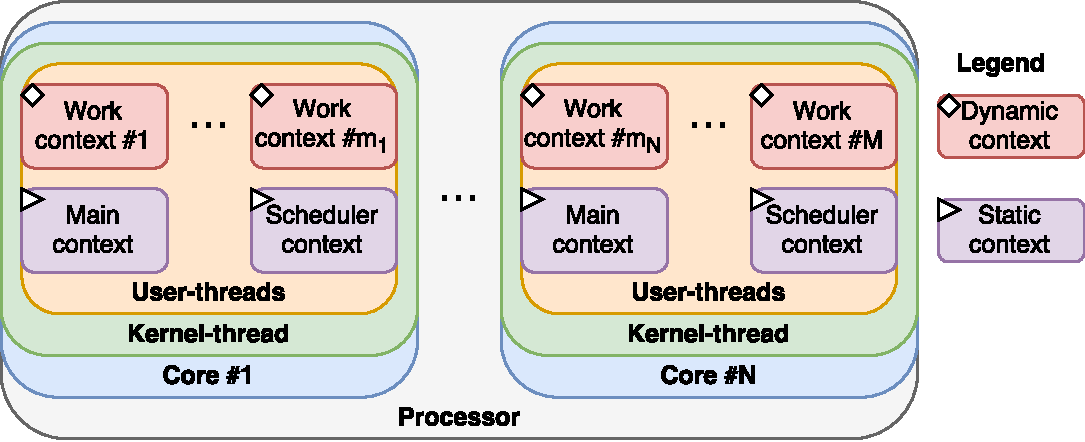
\includegraphics[width=0.9\linewidth]{fig/runtime_overview}
    \caption{Overview of the runtime system with $M$ work contexts, given $N$ online processor cores.}
    \label{fig:runtime_overview}
\end{figure}


%%%%%%%%%%%%%%%%%%%%%%%%%%%%%%%%%%%%%%%%
\subsection{Processes}
\label{subsec:process_implementation}


Processes are a vital part of ProXC++. As stated many times before, processes represents some kind of computation of the total program, which in code translates to running a function concurrently with the rest of the system. Constructing a process requires to supply a function pointer and its corresponding arguments. The process object constructs a context object out the function pointer and arguments, and stores an intrusive pointer to the context object as a data member. In other words, the process is no more than an opaque type to a context object. The programmer implicitly creates new contexts through processes, while the scheduler under the hood operates on the contexts. See \cref{lst:process_type} for reference.

\begin{lstfloat}
\begin{lstlisting}[caption={Minimal process type.}, label={lst:process_type}, style={CustomC++}, xleftmargin={4em}]
class Process {
private:
    using CtxPtr = boost::intrusive_ptr<proxc::Context>;
    CtxPtr ctx_ptr_{ nullptr };
public:
    template<typename Fn, typename... Args>
    Process(Fn && fn, Args &&... args);
};
\end{lstlisting}
\end{lstfloat}

The context objects represent the execution state of the computation. Each context object contains an execution context, which is the actual execution state of the computation. The execution context is implemented by the Boost Context library, which encapsulates context switching and manages the associated contexts stack. Note that a context object refers to the context type defined by the runtime system, and execution context refers to the Boost Context object which defines the actual processor state.

The context object encapsulates the execution context with relevant runtime functionality, such as control structure data and context states.

Execution contexts can either create a context of the current running execution context, or takes a function pointer of the type \lstinline[style={CustomC++}]|void(void*)|. Transfer of control flow between execution contexts is done by calling another execution context with the overloaded \lstinline[style={CustomC++}]|void* operator()(void*)| method. Parameter passing is possible through void pointer casting. When transferring control to another execution context, an optional pointer can be passed. If this is the first transfer of control to the execution context, the parameter will be passed as the void pointer argument for the function. Else, the void pointer will be passed as the return value of the transfer of control operator.

\Cref{lst:transfer_control_execution_contexts} gives an example of how execution contexts work. An execution context of the current running context is made, as well as an execution context of a lambda function. The output of the code snippet will print \texttt{main} and \texttt{work} in that order. Refer to the Boost Context documentation for more thorough explanation of the execution context implementation \citep{kowalke2017boost}.

\begin{lstfloat}
\begin{lstlisting}[caption={Transfer of control between execution contexts.}, label={lst:transfer_control_execution_contexts}, style={CustomC++}, xleftmargin={4em}]
using ex_ctx = boost::context::execution_context;
ex_ctx main_ctx{ex_ctx::current()};
ex_ctx work_ctx{[&main_ctx](void* vp){
    std::string* msg = static_cast<std::string*>(vp);
    std::cout << *msg << std::endl;
    // prints `main`
    std::string work_msg{"work"};
    // transfer of control to main_ctx
    main_ctx(static_cast<void*>(&work_msg));
    // never returns
}};
std::string main_msg{"main"};
// transfer of control to work_ctx
void* vp = work_ctx(static_cast<void*>(&main_msg));
std::string* msg = static_cast<std::string*>(vp);
std::cout << *msg << std::endl;
// prints `work`
\end{lstlisting}
\end{lstfloat}

When creating a context object, an enclosing entry function of the type \lstinline[style={CustomC++}]|void(void*)| is created, which calls the received function with its arguments. This entry function, called trampoline, handles the void pointer argument from the execution context, calls the process function, and calls the terminate procedure when the process function returns. This way, all terminating processes can be gracefully resolved by the trampoline invisible to the programmer. Entry functions are created with generic lambdas, allowing to create generic entry function calling over any type of function pointer and arguments. This is explained in further detail in \cref{subsec:scheduler_implementation}.

The context object contains the type of the context, the execution context, the entry function for the particular process, and a pointer to the parent scheduler. Each process also has its own spinlock, used when synchronizing on certain inter\hyp{}process synchronization. Additionally, control data used by the scheduler is stored in the context object, such as intrusive hooks and time points for timed suspension. See \cref{lst:context_type} for a stripped down version of the context class definition.

\begin{lstfloat}
\begin{lstlisting}[caption={Minimal context type.}, label={lst:context_type}, style={CustomC++}, xleftmargin={4em}]
class Context {
private:
    using ExCtxT = boost::context::execution_context;
    using EntryFn = delegate<void(void*)>;
    using TimePointT = std::chrono::steady_clock::time_point;
    ExCtxT ex_ctx_;
    EntryFn entry_fn_{ nullptr };
    proxc::Scheduler * scheduler_ptr_{ nullptr };
public:
    TimePointT time_point_{ TimePointT::max() };
    proxc::Alt * alt_{ nullptr };
    proxc::Spinlock splk_;
    /* intrusive data members */
};
\end{lstlisting}
\end{lstfloat}

The context object does not implement much functionality, other than wrapping the execution context state with additional control structure data and intrusive data members. The functionality is implemented in the scheduler, which is explained in further detail in \cref{subsec:scheduler_implementation}.


%%%%%%%%%%%%%%%%%%%%%%%%%%%%%%%%%%%%%%%%
\subsection{Scheduler}
\label{subsec:scheduler_implementation}

The scheduler is the corner piece of runtime system. It has the sole responsibility of managing the different contexts, including creating, scheduling, and destroying contexts.

\begin{figure}[h!]
    \centering
    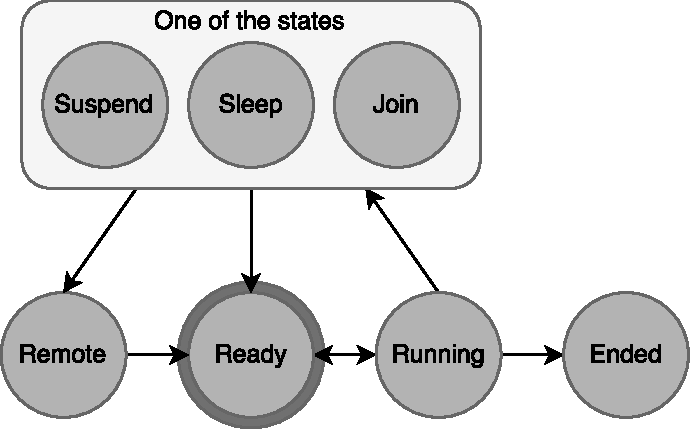
\includegraphics[width=0.7\linewidth]{fig/context_states}
    \caption{Finite state machine of context states and transitions.}
    \label{fig:context_states}
\end{figure}




%%%%%%%%%%%%%%%%%%%%%%%%%%%%%%%%%%%%%%%%%%%%%%%%%%%%%%%%%%%%%%%%%%%%%%%%%%%%%%%%
\section{Library Feature Implementations}

\subsection{Timers}

\subsection{Parallel Statement}

\subsection{Channels}

\subsection{Alting}


\FloatBarrier
%%%%%%%%%%%%%%%%%%%%%%%%%%%%%%%%%%%%%%%%%%%%%%%%%%%%%%%%%%%%%%%%%%%%%%%%%%%%%%%%
\subsection{Scheduler}
\label{subsec:scheduler}
% work stealing
% process create, schedule, join, destroy
% process timeouts

The scheduler runs as its own context, running in an scheduler loop until the program exits. Each spawned kernel\hyp{}thread contains a scheduler context, and the scheduler context never migrates to an another kernel\hyp{}thread. Each scheduler is the ``owner'' of one or more process contexts. ``Owning'' a context is synonymous with management; scheduling, inter\hyp{}process handling, and destroying the context when the corresponding process terminates. When a process is created, the scheduler residing on the same kernel\hyp{}thread ``owns'' that context. Only one scheduler can ``own'' a context at a time.

A scheduler consists of context queues, scheduler functionality, and a scheduler context running an event loop.


\FloatBarrier
%%%%%%%%%%%%%%%%%%%%%%%%%%%%%%%%%%%%%%%%
\subsubsection{Scheduler Event Loop}

The scheduler event loop is the where the entirety of the scheduler context's lifetime executes in. The event loop consists of the following: check of exit flag, context cleanup, context transitions, and context scheduling. See \cref{lst:scheduler_event_loop} for pseudo code reference.

\begin{lstfloat}
\begin{lstlisting}[caption={Scheduler event loop pseudo code.}, label={lst:scheduler_event_loop}, style={CustomC}, xleftmargin={4em}]
void scheduler_event_loop() {
    while ( true ) {
        // check exit flag and break if all workers have finished
        if ( exit_flag ) {
            scheduling_policy.notify();
            if ( work_queue.empty() ) {
                break;
            }
        }
        // cleanup terminated contexts
        cleanup_terminated();
        // transition contexts to ready
        transition_remote(); // remote -> ready
        wakeup_sleep();      // sleep  -> ready
        // schedule ready context if any else wait
        context = scheduling_policy.dequeue();
        if ( context != nullptr ) {
            // scheduler must always be available
            scheduling_policy.enqueue( scheduler_context );
            // context switch to ready context
            resume( context );
            // scheduler is now running
        } else {
            // sleep until first sleeping context timeout
            // or wait until notified
            time_point = ( sleep_queue.empty() )
                ? time_point_max
                : sleep_queue.first() ;
            scheduling_policy.suspend_until( time_point );
        }
    }
    // scheduler is exiting, cleanup scheduler
    scheduler_cleanup();
    // lastly, context switch to main
    resume( main_context );
}
\end{lstlisting}
\end{lstfloat}

\FloatBarrier
%%%%%%%%%%%%%%%%%%%%%%%%%%%%%%%%%%%%%%%%
\subsubsection{Scheduler Functionality}
% framework
% context yield
% context switch data
% context launch
% context joining
% context wait
% context 

Maybe the most important part of the scheduler is context management. The scheduler is responsible for creating new and destroying finished contexts, and 


\FloatBarrier
%%%%%%%%%%%%%%%%%%%%%%%%%%%%%%%%%%%%%%%%
\subsubsection{Context Queues}

Each scheduler has five queues: \textit{ready}, \textit{work}, \textit{sleep}, \textit{terminated}, and \textit{remote} queue. The ready queue holds the set of contexts ready to be scheduled, and is explained in more detail later. The work, sleep and terminated queue is managed only by a single scheduler, and is used to organize the processes the scheduler ``owns''. The work and terminated queues are intrusive doubly linked lists, while the sleep queue is a sorted, intrusive multiset\footnote{A multiset is an associative container that contains a set of objects, which allows multiple keys with the same values.}. The work queue is the total list of all processes the scheduler ``own''. The sleep queue contains all process which are suspended with a given timeout, and are sorted in ascending order. The terminated queue is the queue of all processes which has terminated. The need for this queue will be explained later. 

The remote queue is a concurrent MPSC queue, where the managing scheduler is the consumer while any other schedulers are the producers. Whenever a scheduler readies a context and it does not ``own'' it, the context is placed in the remote queue to the ``owning'' scheduler. The ``owning'' scheduler transitions contexts in the remote queue to the ready queue. In essence, the remote queue is used to signal schedulers when their contexts are readied, since remote schedulers cannot safely access the ready queue.

Now, back to the ready queue. The ready queue, as mentioned above, contains all contexts ready to be scheduled for a given scheduler. Only contexts the scheduler ``owns'' can be enlisted to the ready queue. From the schedulers point of view, the ready queue is a black box. Readied contexts are enqueued to the ready queue, and ready contexts are dequeued when scheduling a new context. How the contexts are stored internally and the policy of what order the contexts are dequeued is determined by the \textit{scheduling policy}. The default scheduling policy in ProXC++ is work stealing, however any other kind of policy could be implemented, such as work sharing and round robin.

The work stealing scheduling policy is implemented as a concurrent double\hyp{}ended SPMC queue, using the design presented in \citet{chase2005dynamic,le2013correct} for efficient non\hyp{}blocking work stealing. The managing scheduler is the producer, while all schedulers are the consumers. The ready queue is responsible for load balancing work between the schedulers. From a schedulers point of view, it cannot tell if a dequeued ready context was stolen or not. It also cannot tell if other ready queues steals from its own ready queue. 

\section{Lightweight Process Implementation}


\section{Scheduler Implementation}

\FloatBarrier
%%%%%%%%%%%%%%%%%%%%%%%%%%%%%%%%%%%%%%%%
\section{Parallel Implementation}
\label{sec:parallel_implementation}

All relevant code for the parallel statement implementation can be found in the following files \texttt{parallel.hpp} and \texttt{process.hpp}.

The parallel statement has two obvious phases: the fork and join phases. 

During the fork phase, each process to be executed in parallel is spawned by the parent process, one by one. This involves creating the process, attaching the process to the current scheduler, and launching the process. Launching the process simply enqueues the process to the ready queue of the current scheduler. When all parallel process has been spawned, the parent process enters the join phase.

The join phase consists of the parent process joining all parallel processes, one by one. Joining a process, which is an atomic operation, involves waiting until the process has terminated. One of two things happen when joining: either the process has not terminated and is still executing, or it has terminated. If the process has terminated, the parent process continues the join phase. If not, the parent process waits. When the process terminates, it will wake up the parent process.

Pseudo code for the parallel implementation is presented in \cref{lst:parallel_statement_pseudo_code}.

\begin{lstfloat}
\begin{lstlisting}[caption={Parallel statement pseudo code.}, label={lst:parallel_statement_pseudo_code}, style={CustomC++}, xleftmargin={4em}]
/* fork phase */
for_each process in parallel_processes {
    process.fork();
}
/* join phase */
for_each process in parallel_processes {
    process.join();
}
\end{lstlisting}
\end{lstfloat}

The parallel statement is quite simplistic, as it only enqueues new processes to the current scheduler and waits for their termination. Much of the simplicity comes from the lack of a \textit{sequential} statement, simplifying the design significantly. 




\section{Timer Implementation}

All relevant code for the timer implementation can be found in the following file \texttt{timer.hpp}.

Timers are represented through a common abstract class interface, shown in \cref{lst:timer_class_interface}. Instances of an egg or repeat timer converts the specified time duration to a time point, while the date timer already specifies a time point. This time point is stored in the base interface class. All timers support duration and time points from the standard library \texttt{std::chrono}.

\begin{lstfloat}
\begin{lstlisting}[caption={Timer class interface.}, label={lst:timer_class_interface}, style={CustomC++}, xleftmargin={4em}]
class timer::Interface {
protected:
    using TimePointT = /* implementation defined */;
    TimePointT time_point_;
public:
    virtual void reset() = 0;
    virtual bool expired() = 0;
    bool operator<( Interface const & other ) const 
    { return time_point_ < other.time_point_; }
    TimePointT const & get() const { return time_point_; }
};
\end{lstlisting}
\end{lstfloat}

When a timer is supplied for a timed operation, the reset method is called. For the egg timer, a reset results in calculating new time point. For the repeat timer, the next periodic time point is calculated if expired, else the time point remains the same.

For some operations, such as alternation, multiple timers can be supplied. Since timers have a static time point after reset, the closest time point is chosen for timeout.

Under the hood, an explicit process suspension with a given timer is simply enlisting the context to the scheduler sleep queue with the corresponding time point. When the time point is reached, the scheduler removes the context from the sleep queue and is rescheduled. The time point is checked by the scheduler context in the \texttt{wakeup\_sleep()} method. If the time point has already reached when suspending the process, it immediately returns. 

A timed operation differs slightly. Whenever the context waits for some event during the operation, the context is enlisted in the scheduler sleep queue. Now, one of two things may happen: either the context is rescheduled by some event, or the operation times out and is rescheduled by the scheduler. If the context was rescheduled by the event, the scheduler removes the context from the sleep queue and is enqueued in the ready queue. If the time point expires, the scheduler transitions the context from the sleep queue to the ready queue in the \texttt{wakeup\_sleep()} procedure. Either way, the context is removed from the sleep queue and enqueued in the ready queue.

Note that if the context is rescheduled by a remote event, the context is enlisted in the remote queue first, but it is not removed from the sleep queue. Its not until the scheduler transitions the context from remote to ready during the \texttt{transition\_remote()} procedure the context is removed from the sleep queue.


\section{Channel Implementation}

All relevant code for channel implementation is found in the file \texttt{channel.hpp} and all files within the folder \texttt{channel/}.

In ProXC++, channels exist in one flavour: synchronous and unbuffered, unidirectional, one\hyp{}to\hyp{}one, and type safe. All channel related objects and methods reside in the \texttt{channel} namespace.

Channels are composed of the two channel end objects \texttt{Tx<T>} and \texttt{Rx<T>}. \texttt{Tx<T>} and \texttt{Rx<T>} can send and receive on a channel, respectively. Channels can only be created through the functions \texttt{create<T>()} for single channel objects, or \texttt{create\_n<T>()} for $n$ channel objects, \cref{lst:channel_create_functions} for reference. 

Channel operations, alting or not, can be timed with a timer. Both sending and receiving channel ends can be used in alternation, compared to occam and XC which only permits receiving channel ends.

Channels can be closed. When a channel is closed, no more channel operations can be completed on the given channel. Closing a channel cannot be undone. A channel closes when either one of the channel ends goes out of scope, or one the channel ends explicitly closes the channel.

\begin{lstfloat}
\begin{lstlisting}[caption={Channel create functions.}, label={lst:channel_create_functions}, style={CustomC++}, xleftmargin={4em}]
template<typename T>
std::tuple< Tx<T>, Rx<T> > create();
template<typename T>
std::tuple< std::vector< Tx<T> >, 
            std::vector< Rx<T> >
> create_n(std::size_t n);
\end{lstlisting}
\end{lstfloat}

\texttt{std::tuple} is used instead of \texttt{std::pair} because \texttt{std::tuple} has better support for metaprogramming, and inline variable definitions are possible with structured bindings in C++17, e.g. \cref{lst:channel_structured_bindings}.

\begin{lstfloat}
\begin{lstlisting}[caption={Creating channels with structured bindings.}, label={lst:channel_structured_bindings}, style={CustomC++}, xleftmargin={4em}]
// until c++17
channel::Tx<int> tx;
channel::Rx<int> rx;
std::tie(tx, rx) = channel::create<int>();
// after c++17
auto [ tx, rx ] = channel::create<int>();
\end{lstlisting}
\end{lstfloat}

Channel ends are movable but non\hyp{}copyable, meaning channel ends must explicitly pass ownership between scopes. As each process in itself is an independent running scope, channel ends being non\hyp{}copyable ensures only one process holds or owns a channel end at any given time. If a process where to pass a channel end to another process, the ownership of the given channel end must be moved.

Channel ends are no more than class object holding a shared pointer to the actual channel object. A shared pointer is a smart pointer which shares ownership to a dynamically allocated object between multiple owners, and which deallocates the object when all owners releases ownership. Channel objects are of type \texttt{ChannelImpl<T>} which contains the entire implementation. Whenever a channel is to be created, a channel object is dynamically allocated with the shared pointer \texttt{std::shared\_ptr<T>}. Additionally, channel ends defines its interface by restricting access to the channel object.

The channel object represents internally each channel end as a struct. This struct contains the context of the calling process, reference to the item being sent or where to store the received item, and pointer to the alternation choice if used in an alternation procedure. See \cref{lst:channel_end_representation} for reference. 

\begin{lstfloat}
\begin{lstlisting}[caption={Channel end representation in channel object.}, label={lst:channel_end_representation}, style={CustomC++}, xleftmargin={4em}]
template<typename ItemT>
struct ChanEnd {
    Context   * ctx_;
    ItemT     & item_;
    AltChoice * alt_choice_;
};
\end{lstlisting}
\end{lstfloat}

The following data members are present in a channel object: A spinlock. Atomic boolean value indicating if the channel is closed or not. An atomic pointer to a channel end struct (\cref{lst:channel_end_representation}), each for Tx and Rx. An atomic boolean used to indicate if an channel end item was consumed by an another channel end or not, each for Tx and Rx. And lastly, an atomic enum used to synchronize between two alting channel ends.

\section{Alting Implementation}

All relevant code is found in the files \texttt{alt.hpp} and \texttt{alt.cpp}, and all files within the folder \texttt{alt/}.

The alting procedure is implemented as a class object, which is allocated on the stack. The channel alternative is composed into two different channel alternative objects, each for the sending and receiving case. Both alternative objects have inherit from a common abstract class interface. The timer and skip alternative is both allocated as a data member in the alting object. 

After creating an alting object, alternatives can be created by chaining function calls to the alting object. The four functions \texttt{send}, \texttt{recv}, \texttt{timeout} and \texttt{skip} creates a channel send, channel receive, timeout and skip alternative, respectively. The channel alternative functions has a corresponding replicator function for creating dynamic number of channel alternatives over a dynamic number of channel ends These are called \texttt{send\_for} and \texttt{recv\_for}. All alternative creating functions also has an corresponding guarded function, which is the function name with \texttt{\_if} appended, e.g. \texttt{send\_if}. Lastly, the function call \texttt{select} performs the alting procedure and consumes the alting object in the process. The \texttt{select} function call is always last. See \cref{lst:code_example_alting} for a code example.

\begin{lstfloat}
\begin{lstlisting}[caption={Code example of alting.}, label={lst:code_example_alting}, style={CustomC++}]
Alt()                           // creates alting object
    .send(tx, item)             // w/o guard, w/o closure
    .recv_if(cond1, rx)         // w   guard, w/o closure
    .timeout(timer, [](){})     // w/o guard, w   closure
    .skip_if(cond2, &some_func) // w   guard, w   closure
    /* more alternatives can be inserted here */
    .select();                  // selects an alternative
\end{lstlisting}
\end{lstfloat}

All of the channel alternative functions simply generate and store alternatives in the alting object. However, some additional care has to be taken into consideration. Multiple alternatives can be created on the same channel end. If this is the case, then the alting object chooses one at random which is used during the alting procedure. If both ends of the same channel is detected as alternatives, then all alternatives for that channel is discarded.

Timeout alternatives are stored as a single entry in the alting object. Whenever a timeout alternative is created, the timeout period is checked against the current timeout period, initialized to maximum value. If the timeout period is lower than the current one, the new timeout alternative is swapped in place.

Skip alternatives are stored as a single entry in the alting object. Compared to the timeout alternative, only the first skip alternative is stored. All subsequent skip alternatives are discarded.

The alting object uses a spinlock to enforce active and passive selection. An atomic flag and a pointer is used to set the ``winner'' of the selection. During the checking phase, the alting object holds the spinlock. If the alting procedure actively selects an alternative, the atomic flag is set and the pointer is set accordingly. Only after alting procedure continues to the waiting or completing phase is the spinlock released. Any alternative that becomes ready during the checking phase and tries to select passively must acquire the alting spinlock first. This allows the alting procedure to enforce all alternatives trying to passively select to wait until the waiting or completing phase. 
If the alting procedure enters the waiting phase, the alting procedure suspends itself and the lock is released. The first alternative to acquire the lock and set the atomic flag is allowed to set the winner pointer. This alternative also reschedules the alting procedure. 

\begin{lstfloat}
\begin{lstlisting}[caption={Code example of alting.}, label={lst:active_alting}, style={CustomC}]
lock = spinlock.aquire();
ready_selected = checking_phase();
winner = if ! ready_selected {
    if skip { skip_alternative }
    else {
        // atomically suspend and release lock
        timeout = scheduler.alt_wait( lock );
        if timeout { timeout_alternative }
        else       { channel_alternative }
    }
} else { ready_alternative };
completing_phase(winner);
\end{lstlisting}
\end{lstfloat}

\begin{lstfloat}
\begin{lstlisting}[caption={Code example of alting.}, label={lst:passive_alting}, style={CustomC}]
lock = spinlock.aquire();
if ! alt.atomic_flag.test_and_set() { return false; }
alt.winner = channel_alternative;
scheduler.reschedule(alt.context);
return true;
\end{lstlisting}
\end{lstfloat}

% FIXME uniform random distribution
% FIXME fairness vs determinism